\documentclass[10pt]{standalone}
\usepackage{commands}

\begin{document}
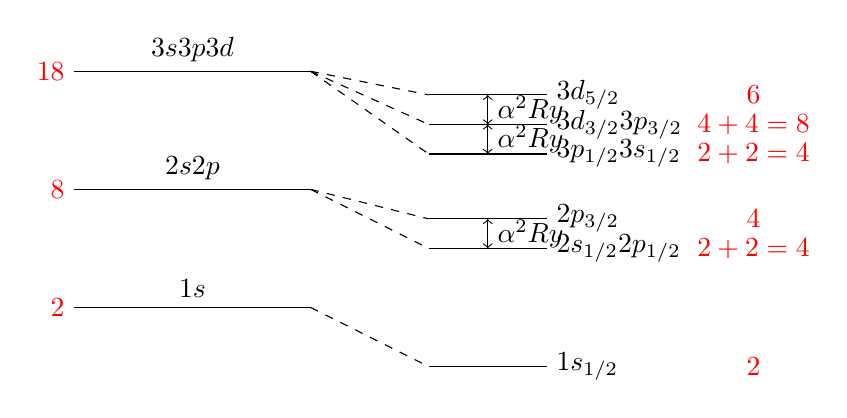
\begin{tikzpicture}[scale=1.5]
    \draw[] (0, 0) -- (2, 0);
    \draw[dashed] (2, 0) -- (3, -0.5);
    \draw[] (3, -0.5) -- (4, -0.5);
    \node[left, red] at (0, 0) {2};
    \node[above] at (1, 0) {$1s$};
    \node[right] at (4, -0.5) {$1s_{1/2}$};
    \node[red] at (5.75, -0.5) {$2$};
    
    \draw[] (0, 1) -- (2, 1);
    \draw[dashed] (2, 1) -- (3, 0.5);
    \draw[] (3, 0.5) -- (4, 0.5);
    \draw[dashed] (2, 1) -- (3, 0.75);
    \draw[] (3, 0.75) -- (4, 0.75);
    \node[left, red] at (0, 1) {8};
    \node[above] at (1, 1) {$2s2p$};
    \node[right] at (4, 0.5) {$2s_{1/2}2p_{1/2}$};
    \node[right] at (4, 0.75) {$2p_{3/2}$};
    \draw[<->] (3.5, 0.5) -- (3.5, 0.75);
    \node[right] at (3.5, 0.625) {$\alpha^2\si{Ry}$};
    \node[red] at (5.75, 0.5) {$2 + 2 = 4$};
    \node[red] at (5.75, 0.75) {$4$};


    \draw[] (0, 2) -- (2, 2);
    \draw[dashed] (2, 2) -- (3, 1.8);
    \draw[] (3, 1.8) -- (4, 1.8);
    \draw[dashed] (2, 2) -- (3, 1.55);
    \draw[] (3, 1.55) -- (4, 1.55);
    \draw[dashed] (2, 2) -- (3, 1.3);
    \draw[] (3, 1.3) -- (4, 1.3);
    \node[above] at (1, 2) {$3s3p3d$};
    \node[left, red] at (0, 2) {18};
    \node[right] at (4, 1.8) {$3d_{5/2}$};
    \node[right] at (4, 1.55) {$3d_{3/2}3p_{3/2}$};
    \node[right] at (4, 1.3) {$3p_{1/2}3s_{1/2}$};
    \draw[<->] (3.5, 1.8) -- (3.5, 1.55);
    \draw[<->] (3.5, 1.55) -- (3.5, 1.3);
    \node[right] at (3.5, 1.425) {$\alpha^2\si{Ry}$};
    \node[right] at (3.5, 1.675) {$\alpha^2\si{Ry}$};
    \node[red] at (5.75, 1.3) {$2 + 2 = 4$};
    \node[red] at (5.75, 1.55) {$4 + 4 = 8$};
    \node[red] at (5.75, 1.8) {$6$};
\end{tikzpicture}
\end{document}